\chapter{Suporte Tecnológico}

Afim de manter e disponibilizar o código e os artefatos gerados a partir deste trabalho, bem como o ambiente utilizado para a construção do framework, serão apresentadas as principais ferramentas candidatas a serem utilizadas durante o seu desenvolvimento.

\section{Ferramentas de Desenvolvimento}

\subsection{Git}

O Git\footnote{\url{https://git-scm.com/}} é um sistema de controle de versão distribuído, projetado basicamente para facilitar a vida de quem quer executar projetos em equipe de forma segura. Foi criado por Linus Torvalds, pois precisava de um controle de versão rápido e que pudesse lidar com uma grande atividade envolvida no desenvolvimento do Kernel do Linux. Linus, desejava um ferramenta livre, não encontrando, ele decidiu criar o Git. Ele foi batizado em referência ao próprio Linus, no inglês britânico, Git é uma gíria para ``cabeça-dura''.

Uma vantagem do Git é a possibilidade de controlar o projeto de forma descentralizada, ou seja, sem a exigência de um servidor mestre. E cada arquivo rastreado pelo Git tem seu conteúdo verificado usando o algoritmo de criptografia SHA-1.

O que faz o Git funcionar mesmo é sua habilidade de detectar mudanças em arquivos, não só que uma mudança ocorreu, mas também onde mudança aconteceu. Podendo desfazer as alterações que estão com problemas, voltando para a versão mais estável.

\begin{figure}[!h]
	\centering
	
\includegraphics[scale=0.35]{figuras/capitulo3/git.eps}
	\caption{Logo do Git}
	\label{git}
\end{figure}

\subsection{GitHub}

O GitHub\footnote{\url{https://github.com}}, lançado 2008 e feito em Ruby on Rails, provê um armazenamento em nuvem (\textit{Cloud}), onde se pode hospedar projetos utilizando o Git como controle de versão. O GitHub possui funcionalidades de um rede social como \textit{feeds}, \textit{followers}, wiki e gráficos para apresentar como os desenvolvedores trabalham em um repositório. Este lado social é interessante para descobrir novos projetos e receber ajuda em projetos particulares. É importante ressaltar que o repositório fornecido pelo GitHub é gratuito. Entretanto, este repositório fica como de acesso público, porém, existem planos comerciais no qual o repositório pode se tornar privado.

\begin{figure}[!h]
	\centering
	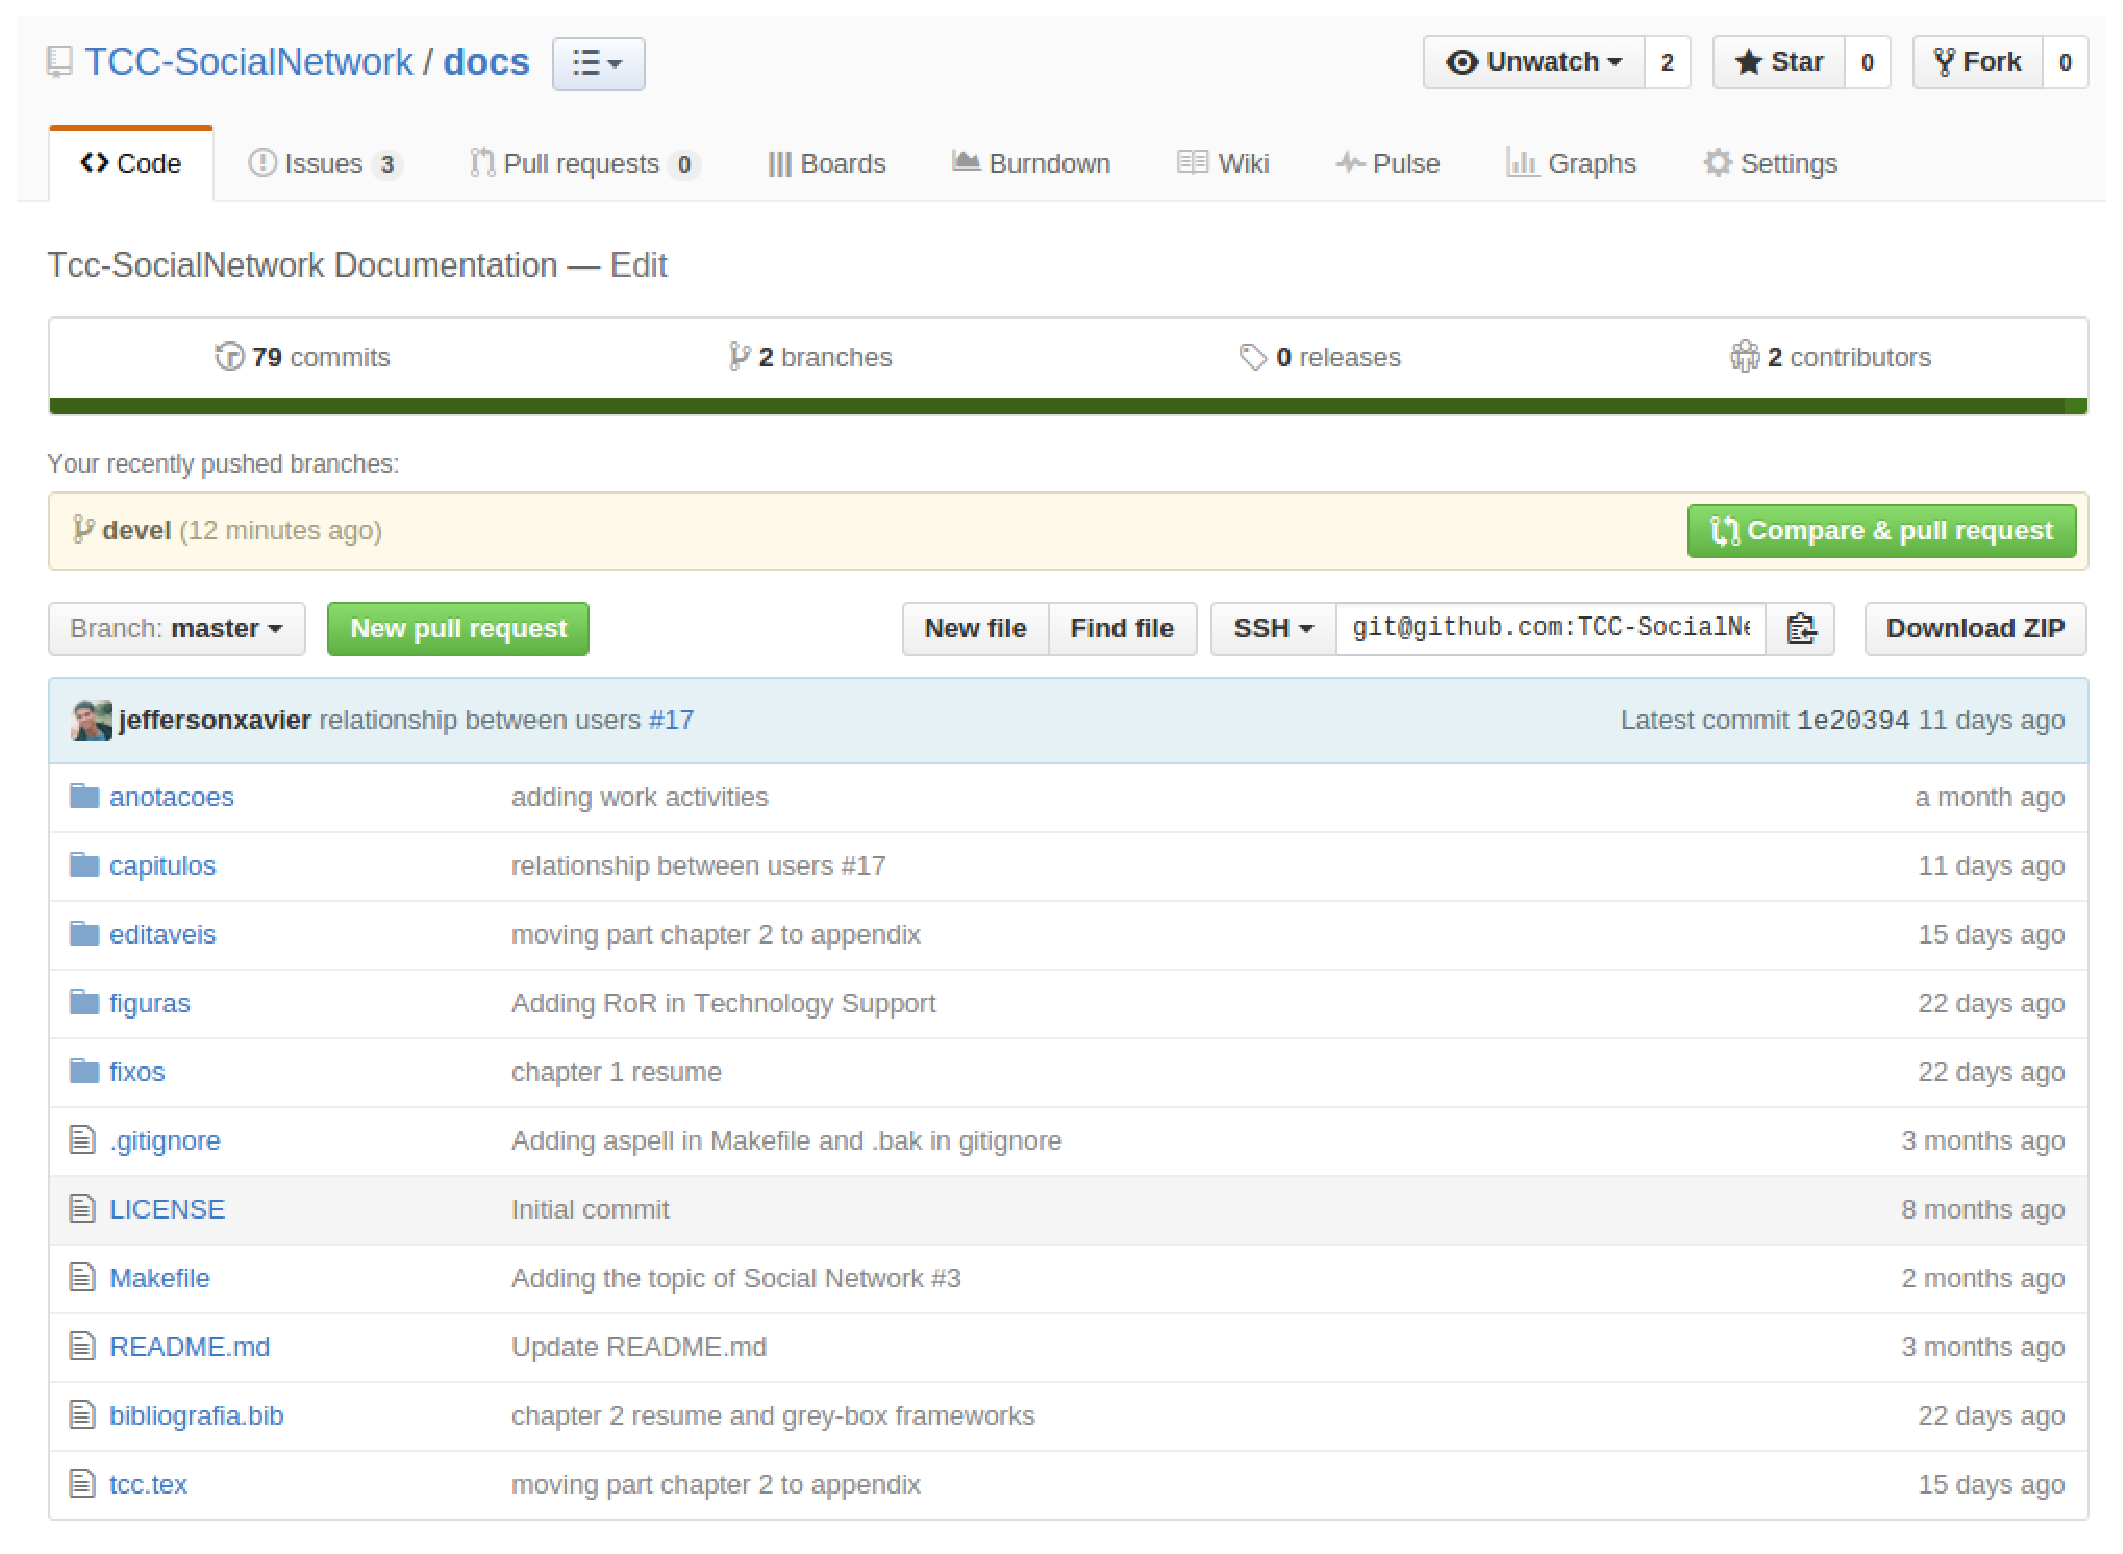
\includegraphics[scale=0.35]{figuras/capitulo3/github.eps}
	\caption{Logo do GitHub}
	\label{github}
\end{figure}

\subsection{ZenHub}

O ZenHub\footnote{\url{https://www.zenhub.io/}}, trata-se de uma extensão para o Chrome para o GitHub, que visa a facilidade as equipes de engenharia a acompanhar o andamento das tarefas de uma forma visual, mostrando-as em um quadro com divisões para cada fase. Com isso pode-se facilmente mover as \textit{issues} entre as fases e acompanhar o andamento do projeto. Outra vantagem em se usar o ZenHub para gerenciar os projetos, é que a sua API pode gerar relatórios, inclusive um \textit{burndown}. O que elimina a necessidade de ferramentas de terceiros de gerenciamento de projeto, criando um local único de foco.

\begin{figure}[!h]
	\centering
	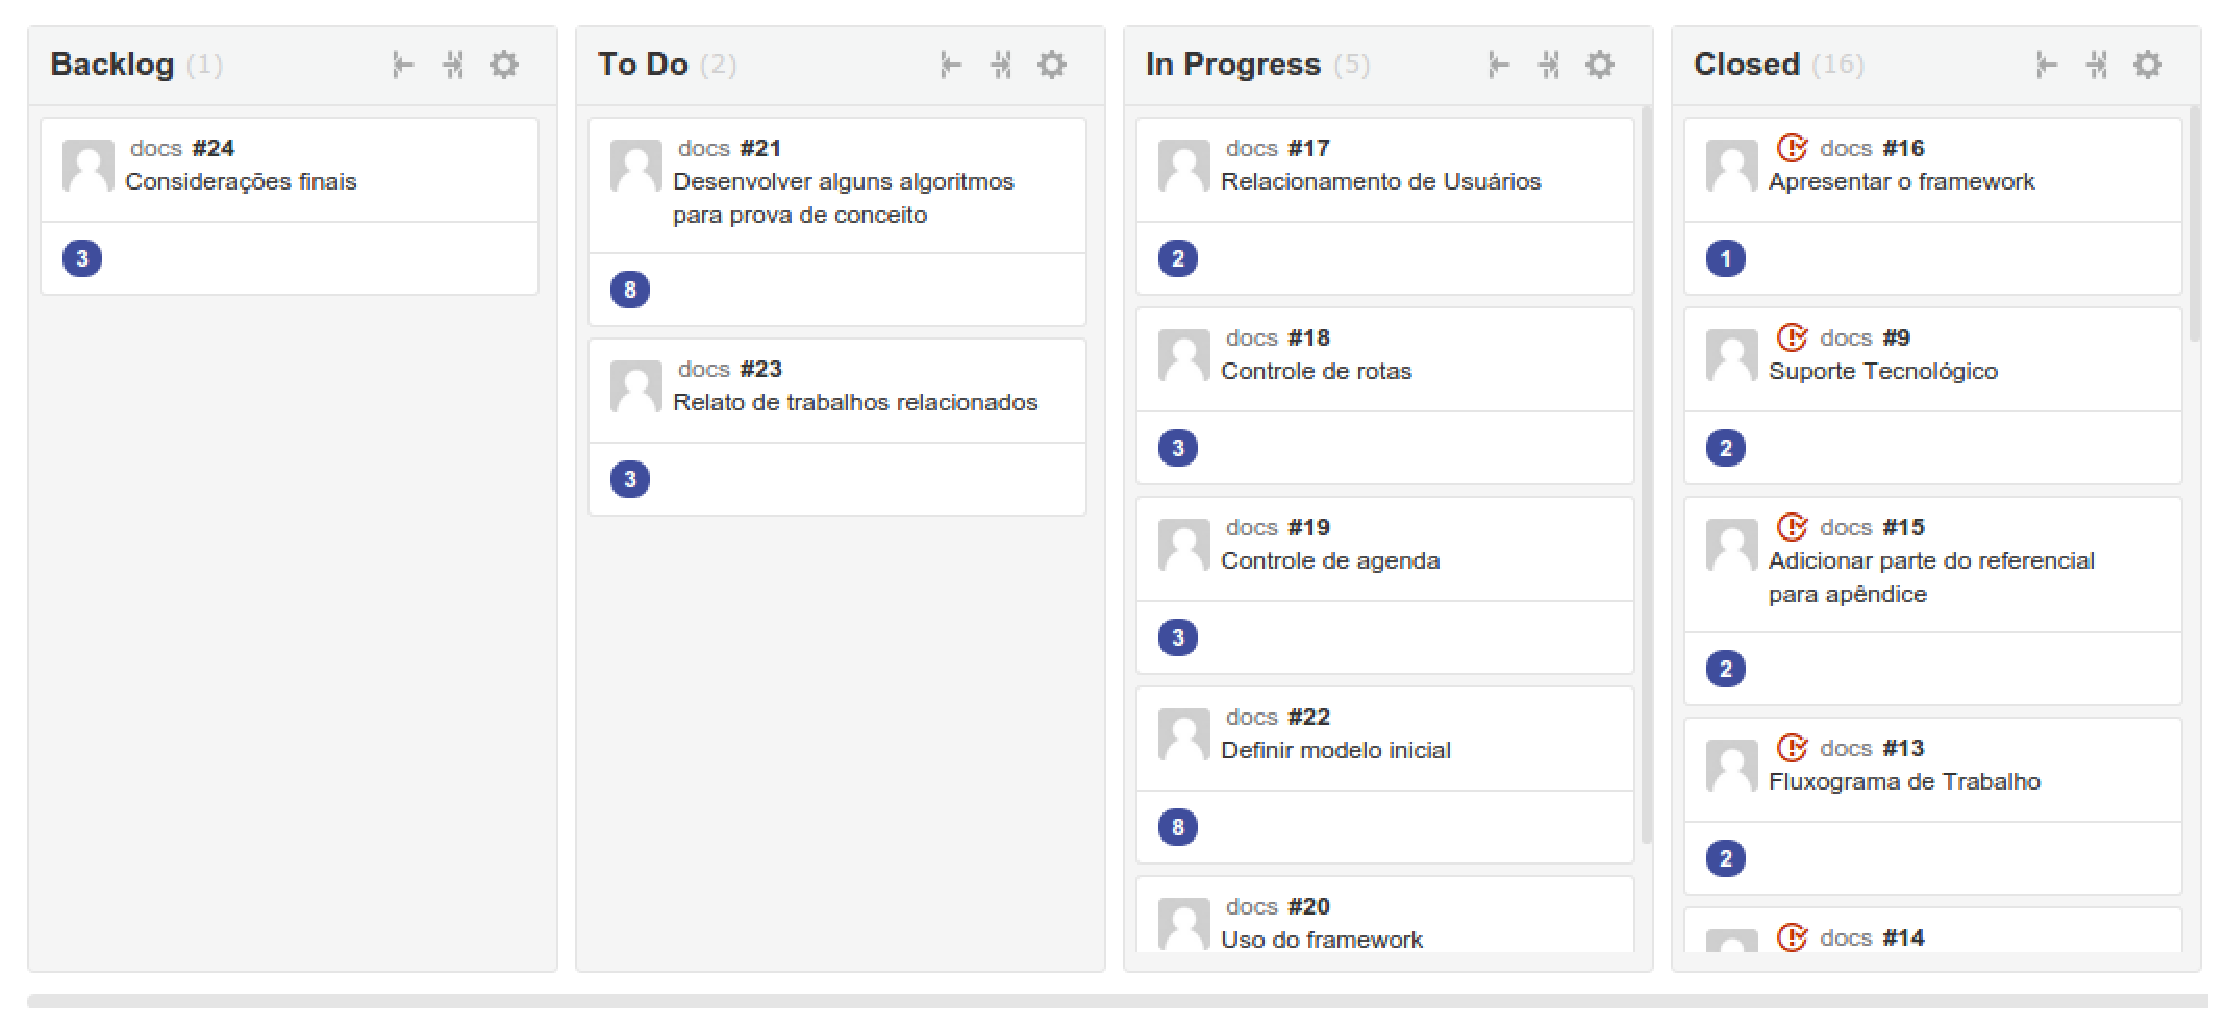
\includegraphics[scale=0.35]{figuras/capitulo3/zenhub.eps}
	\caption{Logo do ZenHub}
	\label{zenhub}
\end{figure}

\subsection{LaTeX}

O \LaTeX\footnote{\url{https://www.latex-project.org}}, é um pacote de macros ou marcações para o processador de textos \TeX. É utilizado amplamente pela comunidade científica devido à sua grande qualidade tipográfica e por torna mais fácil e rápida a produção de documentos em \TeX. O \LaTeX, foi desenvolvido por Leslie Lamport a partir do \TeX, criado por Donald Knuth, e ambos são de código aberto.

O seu objetivo, é que o autor se distancie da apresentação visual do trabalho, e assim, concentrar-se no seu conteúdo. Para isto, ele possui formas de se lidar facilmente com estruturas. Com por exemplo, bibliografias, citações, formatos de páginas e referências. O \LaTeX, não é algo imutável, e como tal, suporta várias maneiras de estilizar e formatar os documentos.

\begin{figure}[!h]
	\centering
	
\includegraphics[scale=0.35]{figuras/capitulo3/latex.eps}
	\caption{Logo do \LaTeX}
	\label{latex}
\end{figure}

\subsection{Sublime Text 3}
\subsection{Bizagi Process Modeler}
\subsection{Linux}
\subsection{C++ ou Ruby}


	ruby
		Cucumber
	c++
		Cunit 
		Analizo - c++
		Sonar - c++
		OCLint - analise estática de código em c/c++
		g++
		gdb

